% small.tex
\documentclass[10pt]{beamer}
\usetheme{amcg}
\beamertemplatenavigationsymbolsempty
\renewcommand{\thefootnote}{}
\providecommand{\e}[1]{\ensuremath{\times 10^{#1}}}
\usepackage{mathptmx}
\usepackage{helvet}
\newcommand\TILDE{\char`\~}
\usepackage{subfigure}
\usepackage{listings}

% items enclosed in square brackets are optional
\title[Introduction to the examples]{Introduction to the examples}
\subtitle[]{}
\institute{Department of Earth Science and Engineering, Imperial College London}
\author[Richard Ferrier]{\large{Richard Ferrier}}
\date{}
\AtBeginSection[]
{
  \begin{frame}
    \frametitle{Outline}
    \tableofcontents[currentsection]
  \end{frame}
}

\begin{document}

%--- the titlepage frame -------------------------%
\begin{frame}
  \titlepage
\end{frame}

%-- Overview slide --- %
\section*{Outline}
\begin{frame}
  \frametitle{Outline}
  \tableofcontents
\end{frame}

\section{CFD Examples}

%\documentclass[10pt]{beamer}
%\usetheme{amcg}
%\usepackage{subfigure}

%\begin{document}

\subsection{Advection of a top hat}

\begin{frame}
  \frametitle{Advection of a top hat}
  \begin{itemize}
  \item Top hat distribution of a tracer, advected with prescribed velocity
  \item Compares CG, CV, DG discretisations
  \item Simple, fast: run time 2 min.
  \end{itemize}

  \begin{figure}
    \centering
    \includegraphics[width=0.45\textwidth]{./top_hat/top_hat_ic.pdf}
    \caption{Initial top hat distribution.}
  \end{figure}
\end{frame}

\begin{frame}
  \frametitle{Advection of a top hat}
  \begin{figure}[ht]
    \begin{tabular}{ccc}
      \includegraphics[width=0.3\textwidth]{./top_hat/top_hat_cg.pdf} &
      \includegraphics[width=0.3\textwidth]{./top_hat/top_hat_cv.pdf} &
      \includegraphics[width=0.3\textwidth]{./top_hat/top_hat_dg.pdf} \\
      Continuous & Control & Discontinuous  \\
       Galerkin &  Volume & Galerkin
    \end{tabular}
  \end{figure}
\end{frame}

\begin{frame}
  Continuous Galerkin
  \begin{itemize}
  \item Basic finite element discretisation
  \item Not good for advection of sharp discontinuities
  \item SUPG stabilisation applied in this instance
  \end{itemize}
  \vspace{5pt}
  Control Volume
  \begin{itemize}
  \item Simple and efficient, sometimes diffusive
  \item Need to choose an interpolation method.  Here, `FiniteElement' interpolation with Sweby limiter is used.
  \end{itemize}
  \vspace{5pt}
  Discontinuous Galerkin
  \begin{itemize}
  \item Popular for advection problems
  \item Slope limiters still needed near discontinuities to prevent overshoots
  \end{itemize}
\end{frame}

\begin{frame}
  \frametitle{Exercises}
  \begin{itemize}
    \item Turn off SUPG stabilisation for the CG case and see what it does.
    \item Change the resolution of the adapted meshes.
    \item Change the temporal and spatial discretisations to get a less diffusive CV advection scheme.
  \end{itemize}
\end{frame}

%\end{document}

%-- Add sections and your outline will be created automatically --%
\section{Lid--Driven Cavity}

% Frame starts a new slide
\begin{frame}
    \frametitle{Lid--Driven Cavity - Setup}
\begin{itemize}
\item Simple test case often used for verification and validation.
\item 2D flow with no slip boundaries on the bottom and sides. Constant rightwards velocity imposed on the lid. 
\item Example file and data are for $Re = 1000$.
\end{itemize}
\begin{figure}
\centering
\includegraphics[width=0.4\textwidth]{./driven_cavity/driven_cavity_streamfunction.png}
\caption{Streamfunction contours in converged solution for $h=1/128$.}
\end{figure}
% end my slide
\end{frame}

\begin{frame}
    \frametitle{Lid--Driven Cavity - Output}
\begin{figure}
\centering
\subfigure[vorticity contours in converged solution for \mbox{$h=1/128$}]{\includegraphics[width=0.35\textwidth]{./driven_cavity/driven_cavity_vorticity.png}}
\hspace{10mm}
\subfigure[error vs. mesh spacing for various metrics from the literature]{\includegraphics[width=0.45\textwidth]{./driven_cavity/driven_cavity_error_plot.png}}
\caption{The error metrics are described in the manual, section 10.4.}
\end{figure}
\end{frame}

\begin{frame}
  \frametitle{Lid--Driven Cavity - Exercises}
\begin{itemize}
\item What about mesh adaptivity?
\item Boundary condition on the lid is set to avoid issues in the upper corners. What happens if we modify this? Use a small mesh first!
\item What happens at higher $Re$?
\item What happens to wall clock time if you run in parallel?
\end{itemize}
\end{frame}







%-- Add sections and your outline will be created automatically --%
\section{Backward facing step}

\begin{frame}
    \frametitle{Backward facing step (2D and 3D)}
\begin{itemize}
\item Classic CFD benchmark test case,
\item Experimental and numerical data available for comparison,
\item Test of numerical methods or turbulence models,
\item Serial and parallel simulations.
\end{itemize}
\begin{figure}
\centering
\includegraphics[width=0.5\textwidth]{./backward_facing_step/backward_facing_step_3d-schematic}
\caption{Geometry of the 3D backward facing step.}
\end{figure}
\end{frame}
%
\begin{frame}
    \frametitle{Backward facing step (2D and 3D)}
\begin{itemize}
\item Simulation run in serial.
\end{itemize}
\begin{figure}
\centering
\includegraphics[width=1.0\textwidth]{./backward_facing_step/backward_facing_step_2d-mesh}
\caption{Geometry of 2D backward facing step showing the mesh.}
\end{figure}
\end{frame}
%
\begin{frame}
    \frametitle{Backward facing step, 2D results}
\begin{itemize}
\item Reattachment point estimation,
\item Profile evolution in time and space.
\end{itemize}
\begin{figure}
\centering
\includegraphics[width=0.7\textwidth]{./backward_facing_step/velocity_profiles_kim_kepsilon}
\caption{Streamwise velocity profiles at several points downstream of the step showing the converged solution.  This is compared to experimental and other numerical data.}
\end{figure}

\end{frame}
%
\begin{frame}
    \frametitle{Backward facing step, 3D results}
\begin{itemize}
\item Recirculation bubble and reattachment point.
\end{itemize}

\begin{figure}
\centering
\includegraphics[width=0.8\textwidth]{./backward_facing_step/velo-magnitude-3d-50sec}
\caption{The velocity on a cut plane through the centre of the 3D geometry, time $=50\,$s.}
\end{figure}

\end{frame}
%
\begin{frame}
    \frametitle{Backward facing step, exercises}
\begin{itemize}
\item Increase the Reynolds number.
\item Add adaptivity options for both 2D and 3D.
\end{itemize}

\end{frame}

%\documentclass[10pt]{beamer}
%\usetheme{amcg}

%\begin{document}

\section{Flow past a sphere}

\frame{
  \frametitle{Flow past a sphere}
  \begin{itemize}
    \item Fluidity is used compute the drag force on an isolated sphere, see Chapter 10.7.2 and Equation (10.2) in the manual for more details.\newline
    %\begin{equation}
    %  \label{eq:drag_coefficient}
    %  C_D = \frac{F_x}{\frac{1}{2} \rho u_0^2 A}, \;\;\; \text{with} \;\;\; F_x = \int_S (n_x p - n_i\tau_{ix})dS
    %\end{equation}
    \item The results are compared against a curve optimised to fit a large amount of experimental data (Brown and Lawler, 2003), see Chapter 10.7.3 and Equation (10.3) in the manual for more details.\\
    %\begin{equation}
    %  \label{eq:drag_coefficient_brown2003}
    %  C_D = \frac{24}{Re}(1+0.15Re^{0.681}) + \frac{0.407}{1+\frac{8710}{Re}}
    %\end{equation}
  \end{itemize}
  
}

\frame{
  \frametitle{Flow past a sphere - Setup}
  \begin{itemize}
    \item The sphere is modelled as a void space in the mesh.\newline
    \item The flow is assumed to be incompressible\newline
    \item Free-slip boundary conditions are applied to the top, bottom and side walls, and a no-slip condition to the surface of the sphere.
  \end{itemize}
}

\frame{
  \frametitle{Flow past a sphere - Computational domain}
  \begin{figure}[h]
    \centering
    \includegraphics[scale=0.22]{flow_past_sphere/images/domain_yz.png}\quad\includegraphics[scale=0.22]{flow_past_sphere/images/domain_xy.png}
  \end{figure}
}

\frame{
  \frametitle{Flow past a sphere - Results}
  \begin{figure}
  \centering
    \subfigure{
    \includegraphics[scale=0.0425,clip]{flow_past_sphere/images/sphere-Re1-streamlines.png}}
    \subfigure{
    \includegraphics[scale=0.0425,clip]{flow_past_sphere/images/sphere-Re10-streamlines.png}}
    \\
    \subfigure{
    \includegraphics[scale=0.0425,clip]{flow_past_sphere/images/sphere-Re100-streamlines.png}}
    \subfigure{
    \includegraphics[scale=0.0425,clip]{flow_past_sphere/images/sphere-Re1000-streamlines.png}}
    \caption{Streamlines and surface mesh in the flow past the sphere example. Top-left to bottom-right
    show results from Reynolds numbers $Re=1,10,100,1000$.}
  \end{figure}
}

\frame{
  \frametitle{Flow past a sphere - Results}
  \begin{figure}
  \centering
  \includegraphics[scale=1]{flow_past_sphere/images/Sphere_Drag}
  \end{figure}
}

\frame{
  \frametitle{Flow past a sphere - Exercises}
  \begin{itemize}
    \item We actually compute the (vector) force on the sphere and output this to the stat file. This can then be converted to the drag coefficient via (10.2). Write a Python function to do this conversion and the error from the correlation (10.3).\newline
    \item Try varying some of the discretisation and adaptivity parameters to see what the impact on the accuracy of the calculated drag is.\newline
    \item Try changing the shape of the object, e.g.~benchmark data is also available for flow past a cylinder [Sch\"{a}fer et al., 1996].
  \end{itemize}
}

%\end{document}

%\documentclass[10pt]{beamer}
%\usetheme{amcg}

%\begin{document}

\section{Water collapse}

\frame{
  \frametitle{Water collapse}
  \begin{itemize}
    \item Fluidity is used to replicate a laboratory experiment of a collapsing column of water within an atmosphere of air (Lakehal et al., 2002).\newline
    \item A reservoir of water is initially held behind a barrier.\newline
    \item The water column collapses and floods the rest of the tank when the barrier is quickly removed.
  \end{itemize}
}

\frame{
  \frametitle{Water collapse - Simulation setup}
  \begin{itemize}
    \item The multi-material approach is used to represent the two fluids.
    \item The flow is assumed to be incompressible, inviscid, and 2D.
    \item Free-slip boundary conditions on the bottom and sides, and open top.
  \end{itemize}
        \hspace{-.05\textwidth}
 \includegraphics[scale=0.23]{./water_collapse/setup1.pdf}
 \includegraphics[scale=0.23]{./water_collapse/setup2.pdf}
}

\frame{
  \frametitle{Water collapse - Numerical results (1)}
\begin{figure}[H]
        \centering
 \includegraphics[scale=0.28]{./water_collapse/results1.pdf}
\end{figure}
}

\frame{
  \frametitle{Water collapse - Numerical results (2)}
        \vspace{-.025\textwidth}  
\begin{figure}[H]
        \centering
  \includegraphics[scale=0.25]{./water_collapse/results2.pdf}
\end{figure}
}

\frame{
  \frametitle{Water collapse - Exercises}
 \begin{itemize}
    \item Disable the adaptivity option to run on a fixed mesh.\newline
    \item Alter the water/air viscosity/density.\newline
    \item Modify the tank geometry.
 \end{itemize}
}

%\end{document}

%-- Add sections and your outline will be created automatically --%
\subsection{Tephra settling}

% Frame starts a new slide
\begin{frame}
  \frametitle{Tephra settling}
  \begin{itemize}
    \item Fluidity is used to replicate a laboratory experiment of tephra (fine volcanic ash
particles) settling through a tank of water (Carey, 1997).\newline
    \item Small tephra particles can settle either individually, or collectively as a cloud of particles (a plume).\newline
    \item Plumes are generated when the bulk density of the tephra-water mixture becomes large enough, yielding settling velocities much greater than those expected of single particles (which settle at a velocity given by Stokes law).
  \end{itemize}
\end{frame}

\begin{frame}
  \frametitle{Tephra settling - Simulation setup}
  \begin{itemize}
    \item The simulation uses a 0.3 x 0.7 metre domain, replicating the cross-section of the water tank used in the experiments.\newline
    \item No normal flow boundary conditions are weakly imposed along with a zero velocity initial condition, and the initial volume fraction of the particle phase is set to $1.0 \times 10^{-7}$.\newline
    \item The influx of particles from the air above is simulated using a \texttt{flux} boundary condition at the top of the domain. This allows tephra to flux in at a rate of $0.472\ \mathrm{gm^{-2}s^{-1}}$.
  \end{itemize}
\end{frame}

\begin{frame}
  \frametitle{Tephra settling - Numerical results (1)}
\begin{figure}[H]
        \centering
                \includegraphics[scale=0.2]{tephra_settling/tephra_fine_1.png}\hspace{0.1cm}
                \includegraphics[scale=0.2]{tephra_settling/tephra_fine_2.png}\hspace{0.1cm}
                \includegraphics[scale=0.2]{tephra_settling/tephra_fine_3.png}\hspace{0.1cm}
                \includegraphics[scale=0.2]{tephra_settling/tephra_fine_4.png}\hspace{0.1cm}
                \includegraphics[scale=0.2]{tephra_settling/tephra_fine_5.png}
   \label{fig:tephra_adaptive}
   \caption{Simulation visualisations at $t = 10, 30, 50, 80$ and $110$ seconds. Tephra particles initially settle individually, but as more tephra fluxes in, the layer eventually becomes unstable and plumes begin to form.}
\end{figure}
\end{frame}

\begin{frame}
  \frametitle{Tephra settling - Numerical results (2)}
\begin{figure}[H]
        \centering
                \includegraphics[scale=0.27]{tephra_settling/tephra_velocity.pdf}
   \label{fig:tephra_velocity}
   \caption{Plot of the maximum tephra phase velocity against time. Tephra particles initially settle at approximately $0.0017\ \mathrm{ms^{-1}}$, as predicted by Stokes' law. Plumes begin to form after approximately 30 seconds, resulting in settling velocities over 10 times greater than that of an individual particle.}
\end{figure}
\end{frame}

\begin{frame}
  \frametitle{Tephra settling - Exercises}
 \begin{itemize}
    \item Decrease the characteristic element size to better resolve the plume behaviour.\newline
    \item Alter the particle size to observe its effect on plume formation.\newline
    \item Add a second particle phase (with a different particle size).
 \end{itemize}
\end{frame}




\addtocontents{toc}{\newpage}

\section{GFD Examples}

%-- Add sections and your outline will be created automatically --%
\subsection{The lock--exchange}

% Frame starts a new slide
\begin{frame}
    \frametitle{The lock--exchange}
\begin{itemize}
\item Fluids of different densities (temperature) separated by a barrier. As the barrier is removed, the denser fluid
  collapses under the lighter.
\item Boussinesq flow, control volume discretisation, mesh adaptivity
\item Run time: 10 min.
\end{itemize}

\begin{figure}
\centering
\includegraphics[width=0.45\textwidth]{./lock_exchange/le_basic_0_T}
\caption{Lock-exchange initial temperature (colour) distribution.}
\end{figure}

\end{frame}
%
\begin{frame}
    \frametitle{The lock--exchange}
\begin{figure}[ht]
  \centering
  % For some reason tex4ht doesn't like these images.
  \subfigure[$t = 0\,$s]{\includegraphics[width=0.45\textwidth]{./lock_exchange/le_basic_0_T}}
  \subfigure[$t = 0\,$s]{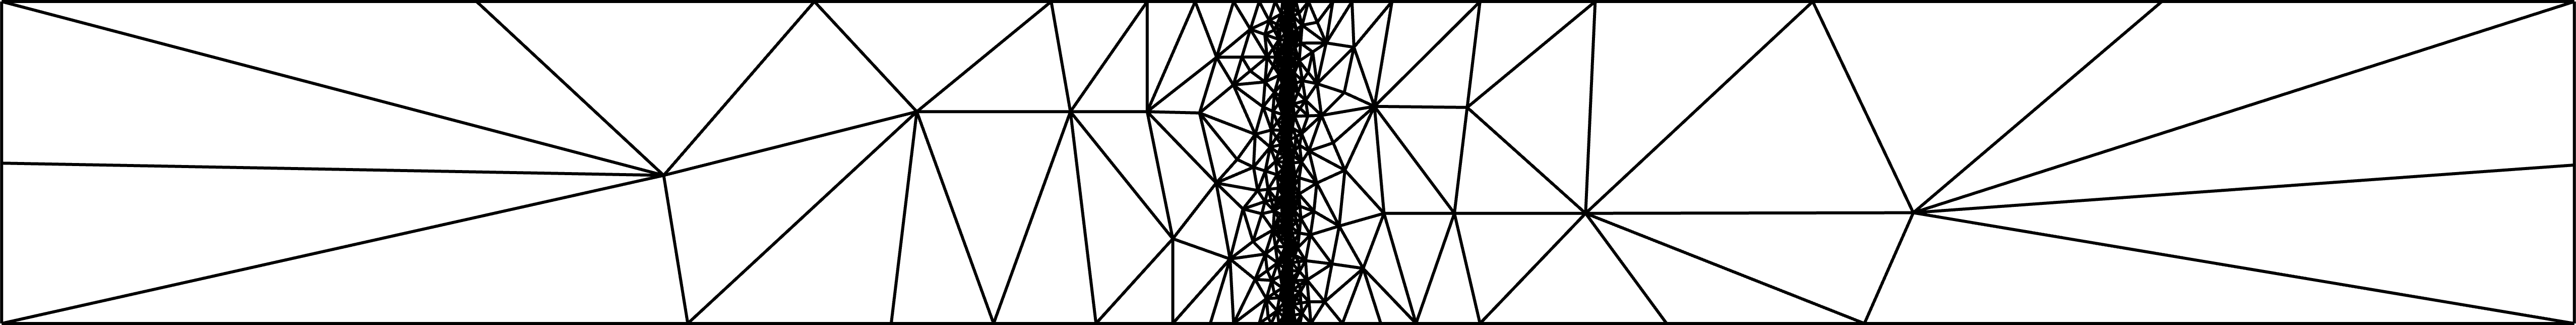
\includegraphics[width=0.45\textwidth]{./lock_exchange/le_basic_0_mesh_nice}} \\
  \subfigure[$t = 12.475\,$s]{\includegraphics[width=0.45\textwidth]{./lock_exchange/le_basic_10_T}}
  \subfigure[$t = 12.475\,$s]{\includegraphics[width=0.45\textwidth]{./lock_exchange/le_basic_10_mesh}} \\
  \subfigure[$t = 37.475\,$s]{\includegraphics[width=0.45\textwidth]{./lock_exchange/le_basic_30_T}}
  \subfigure[$t =
  37.475\,$s]{\includegraphics[width=0.45\textwidth]{./lock_exchange/le_basic_30_mesh}}
  \caption{Lock-exchange temperature distribution (colour) with meshes, over time ($t$).}
\end{figure}
\end{frame}
%
\begin{frame}
    \frametitle{The lock--exchange, diagnostics}
\begin{itemize}
\item Front speed (or Froude number)
\item Mixing given by domain fraction of fluid in specified temperature classes
\end{itemize}

\begin{figure}
\centering
\includegraphics[width=0.5\textwidth]{./lock_exchange/mixing}
\caption{Time evolution of fraction of domain that contains fluid in three temperature classes. Blue: cold, red: warm, green : mixed}
\end{figure}

\end{frame}
%
\begin{frame}
    \frametitle{The lock--exchange, exercises}
\begin{itemize}
\item Increase the simulation time from the default settings (to e.g. 30 secs) and calculate the average Froude number
\item Play with the adaptivity options.
\item Change the diffusivity and viscosity values.
\item Run with a fixed mesh (this will require making a new input mesh)
\item Try adding some detectors to visualise the particle trajectories.
\end{itemize}

\end{frame}

%-- Add sections and your outline will be created automatically --%
\section{Tsunami}

% Frame starts a new slide
\begin{frame}
    \frametitle{Hokkaido-Nansei-Oki tsunami}
\begin{minipage}[]{0.5\linewidth} 
\begin{itemize}
\item Okushiri island, Japan, 1993. 
\item Runup height of up to 30m.
\item Simulation based on a 1:400 laboratory setup.
\item Uses the free-surface and wetting and drying functionality of Fluidity.
\end{itemize}
\end{minipage}
\hspace{0.5cm}
\begin{minipage}[]{0.4\linewidth} 
\begin{figure}
\begin{center}
\includegraphics[width=\textwidth]{hokkaido-nansei-oki_tsunami/MonaiValleyDomainWithInputWave2_png.pdf}
\end{center}
\caption{The domain and the three gauge stations.}\label{fig:monai_inputwave}
\end{figure}
\end{minipage}
\end{frame}

\begin{frame}
    \frametitle{Hokkaido-Nansei-Oki tsunami}
\begin{figure}
\begin{center}
\includegraphics[width=0.7\textwidth]{hokkaido-nansei-oki_tsunami/MonaiValley_C_p1p1_nu0_01_kmkstab_drag0_002_butcircularoundisland0_2-crop-crop_final2.pdf}
\caption{The numerical and experimental results at the three gauge stations.}\label{fig:monai_results}
\end{center}
\end{figure}
% end my slide
\end{frame}


\begin{frame}
    \frametitle{Hokkaido-Nansei-Oki tsunami - Exercises}
  \begin{itemize}
    \item Add more detectors.\newline
    \item Check how increasing the wetting and drying threshold parameter affects the results.\newline
    \item Try changing the viscosity value (How does it affect the inundation of the tsunami event?).
  \end{itemize}
% end my slide
\end{frame}



%-- Add sections and your outline will be created automatically --%
\subsection{Rotating periodic channel}

% Frame starts a new slide
\begin{frame}
    \frametitle{Rotating periodic channel}
\begin{itemize}
\item Unit square domain, periodic in zonal direction and zero-slip at North and South boundaries.  Coriolis forcing.
\item The flow is driven by a velocity source term:
\begin{equation*}
  \vec{F}=
  \begin{bmatrix}
    y^3 \\
    0
  \end{bmatrix}
\end{equation*}
\item Provides a convergence test for the $P_{1DG}P_2$ element pair.
\item A good example of using python state for online diagnostics and analysis, and also using python for setting initial conditions.
\item Run time: 10 min. 
\end{itemize}
\end{frame}
%
\begin{frame}
    \frametitle{Rotating periodic channel}
\begin{figure}
\includegraphics[width=0.6\textwidth]{./rotating_channel/analytic_solution}
\caption{Velocity forcing term and analytic solutions for velocity and pressure for the rotating periodic channel test case. Note that each of these quantities is constant in the x direction.}
\end{figure}
\end{frame}
%
\begin{frame}
    \frametitle{Rotating periodic channel}
\begin{figure}
\includegraphics[width=0.6\textwidth]{./rotating_channel/convergence}
\caption{Error in the pressure and velocity solutions for the rotating channel as a function of resolution.}
\end{figure}
\end{frame}
%
\begin{frame}
    \frametitle{Rotating periodic channel, exercises}
\begin{itemize}
\item Understand the use of analytic forcing functions in Fluidity using Python.
\item For the Continuous Galerkin example, see what the effect is of removing the SUPG stabilisation
\item Change the resolution of the adapted meshes
\item Change the spatial and temporal discretisations to get a less diffusive advection scheme
\end{itemize}
\end{frame}


%-- Add sections and your outline will be created automatically --%
\section{Restratification following open ocean deep convection}

% Frame starts a new slide
\begin{frame}
    \frametitle{Restratification following open ocean deep convection}
\begin{itemize}
\item Idealised model of the restratification phase of OODC using $P_1DGP_2$ using an extruded mesh.
\end{itemize}
\begin{figure}
\includegraphics[width=0.5\textwidth]{./restratification_after_oodc/rousset-init.png}
\caption{A vertical slice throughout the domain showing the initial temperature stratification. The domain is a cylinder of radius $250 \,$km and height $1\,$km.}
\end{figure}
\end{frame}
%
\begin{frame}
    \frametitle{Restratification following open ocean deep convection}
\begin{figure}
\centering
\subfigure [0 days]{\includegraphics[width=0.175\textwidth]{./restratification_after_oodc/rousset-res5000-depth-40m0001.png}}
\subfigure [10 days]{\includegraphics[width=0.175\textwidth]{./restratification_after_oodc/rousset-res5000-depth-40m0003.png}}
\subfigure [20 days]{\includegraphics[width=0.175\textwidth]{./restratification_after_oodc/rousset-res5000-depth-40m0005.png}}
\subfigure [30 days]{\includegraphics[width=0.175\textwidth]{./restratification_after_oodc/rousset-res5000-depth-40m0007.png}}
\subfigure [40 days]{\includegraphics[width=0.175\textwidth]{./restratification_after_oodc/rousset-res5000-depth-40m0009.png}}
\caption{The temperature cross section at a depth of $40\,$m.}
\end{figure}
\end{frame}
%
\begin{frame}
    \frametitle{Restratification following open ocean deep convection, exercises}
\begin{itemize}
\item Work out the kinetic and potential energies using the vtus or stat file.
\item Try running with different resolutions and look at the effect on the eddies.
\end{itemize}
\end{frame}


%-- Add sections and your outline will be created automatically --%
\section{Tides in the Mediterranean Sea}

% Frame starts a new slide
\begin{frame}
    \frametitle{Tides in the Mediterranean Sea}
\begin{itemize}
\item Tidal modelling is a widely used method for validating free surface implementations.
\item Tides introduced by an astronomical body forcing, and a
\item Co--oscillating boundary tide forcing.
\item This example considers the four main tidal constituents: \mbox{$M_2, \, S_2, \, K_1 \,\, {\rm and} \,\, O_1$}.
\end{itemize}
\end{frame}
%
\begin{frame}
    \frametitle{Tides in the Mediterranean Sea}
\begin{figure}
\centering
\includegraphics[width=0.9\textwidth, clip = True, trim = 5mm 180mm 0mm 0mm]{./tides_in_the_Mediterranean_Sea/amp.png}
\caption{The $M_2$ tidal harmonic amplitude from (left) Fluidity--ICOM and (right) a high resolution tidal model${}^\dagger$.}
\end{figure}
\footnote{${}^\dagger$ M.~N.~Tsimplis {\it et al.} (1995), J. Geophys. Res. 100 (C8).}
\end{frame}
%

\begin{frame}
    \frametitle{Tides in the Mediterranean Sea}
The amplitude of each of the todal components is considered, and a RMS error of the difference of these to observed tide guage data is calculated.  The locations of these tide guages is shown below.
\begin{figure}
\centering
\includegraphics[width=0.6\textwidth]{./tides_in_the_Mediterranean_Sea/gauges.png}
\caption{Locations of 62 tide gauges in the Mediterranean Sea used to calculate the root mean square error.}
\end{figure}
\end{frame}


\begin{frame}
    \frametitle{Tides in the Mediterranean Sea - exercises}
\centering
\begin{itemize}
\item Consider the forcing tidal components contained in the netCDF file 'med.nc' (e.g. using ncview).
\item Examine the mesh features (e.g. open the '.msh' file in Gmsh).
\item Look at how to apply the forcing of different tidal components in the simulation.
\item Limit the error calculation by region, are the errors greater in some parts of the Mediterranean?
\end{itemize}
\end{frame}

%-- Add sections and your outline will be created automatically --%
\section{Stokes square convection}

% Frame starts a new slide
\begin{frame}
    \frametitle{Stokes square convection}
\begin{itemize}
\item A steady–state isoviscous convection at a Rayleigh number (Ra) of $10^5$ , in a
  two dimensional square domain of unit dimensions 
\item comparison of numerical results against a well established two dimensional cartesian geometry
  benchmark result for Stokes flow
\end{itemize}
\end{frame}

\begin{frame}
    \frametitle{Stokes square convection}
\begin{figure}
  \includegraphics[width=0.5\textwidth]{./stokes_square_convection/Temperature_planform.png}
  \caption{Steady–state temperature field from an isoviscous Stokes simulation at $Ra = 1 \times
    10^5$, on a uniform structured mesh of 48 × 48 elements. Contours are spaced at intervals of
    0.1.}
\end{figure}
\end{frame}
%
\begin{frame}
    \frametitle{Stokes square convection}
\begin{figure}
\centering
\includegraphics[width=0.5\textwidth]{./stokes_square_convection/Nu_1e5.png}
\includegraphics[width=0.5\textwidth]{./stokes_square_convection/RMS_1e5.png}
\caption{Results from 2-D, isoviscous Stokes square convection benchmark cases: (a) Nusselt number
  vs. number of triangle vertices, at $Ra = 1 \times 10^5$, (b) RMS velocity vs. number of triangle
  vertices, at $Ra = 1 \times 10^5$ . Benchmark values are denoted by horizontal dashed lines. Note that the
  highest resolution case is not included in the example.}
\end{figure}
\end{frame}
%
\begin{frame}
    \frametitle{Stokes square convection, exercises}
\begin{itemize}
\item Verify that results do indeed converge towards the benchmark values at higher resolution.
\item Alter the initial condition for temperature to verify that, excluding the location of upwelling
flow at $x = 0$ or $x = 1$, results are insensitive to this initial condition.
\item Change the Rayleigh number to $Ra = 1 \times 10^4$
\end{itemize}
\end{frame}



\section*{Getting started}
\begin{frame}
  \frametitle{Getting started}
  \begin{itemize}
  \item The examples have been run in advance and the output can be found in \texttt{/scratch/examples}
  \item You may need to specify your Fluidity binaries folder \\
    \texttt{export PATH=<<fluidity dir>>/bin/:\$PATH}
  \item and Python tools folder \\
    \texttt{export PYTHONPATH=<<fluidity dir>>/python/:\$PYTHONPATH}
  \item If you get `permission denied' running a postprocessing script, try \\
    \texttt{chmod u+x <<script>>}
  \end{itemize}
\end{frame}

\end{document}




